% three_pi.tex
% by Troy Hix, April 2005
%----------------------------------------------------------------------------
\begin{figure}
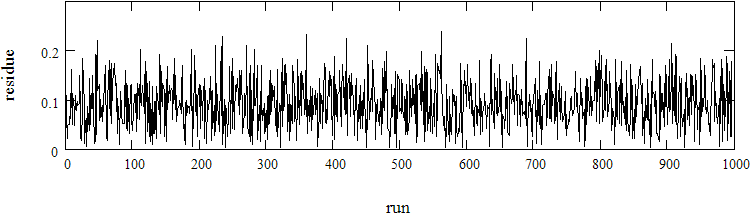
\includegraphics[width=6.00in]
{three_pi/three_pi.png}\\
\caption[Residue for runs using three $\pi$ pulses]{Residue for runs using three $\pi$ pulses. Three pulses of the form shown is figure \ref{solution one} were used at $t_\alpha=5$, $t_\beta=15$, and $t_\gamma=25$. The pulse amplitudes $A$, $B$, and $C$ varied uniformly on the interval $[-20\%,+20\%]$ for 1000 runs.}
\label{three pi}
\end{figure} 
%----------------------------------------------------------------------------
%
